\chapter{Exercise 1 - Equation solving}
\paragraph{1.1}
\begin{wrapfigure}[6]{r}{0.35\textwidth}
\flushright
    \centering
    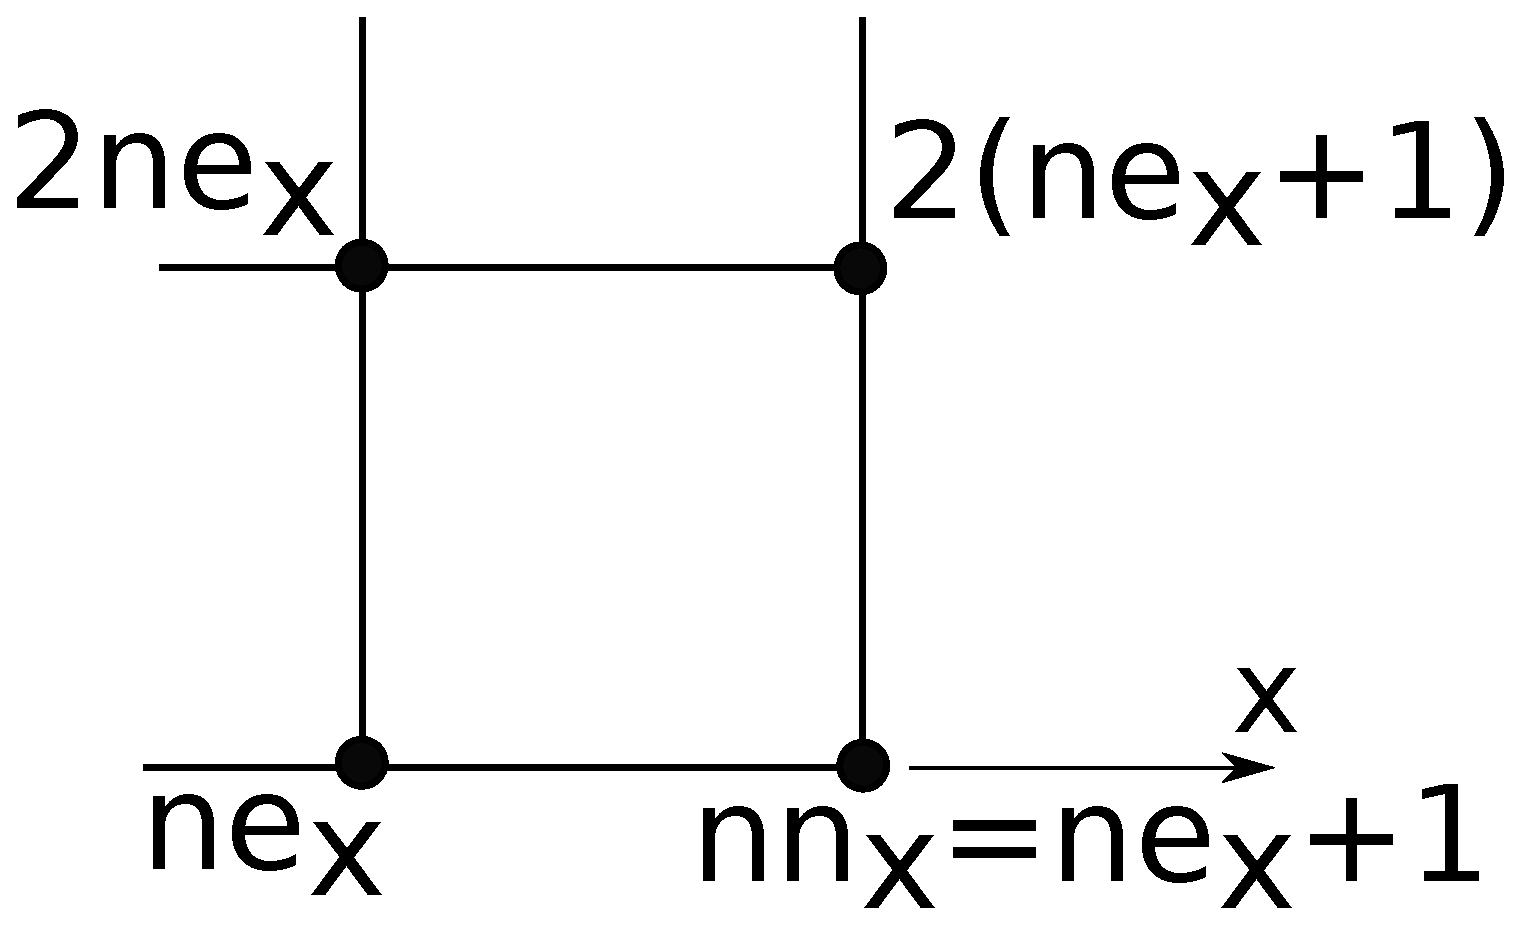
\includegraphics[trim=.0cm .0cm .0cm .0cm, clip=true,width=0.20\textwidth]{Figures/BWfuncofnex.eps}
\caption{Element in bottom right corner}
\label{fig:meshcorner}
\end{wrapfigure}
The bandwidth is expected to increase with the amount of elements in the x-direction and thus giving a higher computational time. 
Considering the order of node numbering the bandwidth can be determined as a function of $\text{ne}_x$ from \Cref{fig:meshcorner}. $bw=2 \text{ne}_x+6$.
Meshes with an even distribution of elements have a lower neqn because of having more nodes that are shared among 4 elements and fewer edge-nodes only shared by 2 elements.
The difference in computation time can be estimated from the amount of multiplication operations required for solving the system of equations. For a banded matrix the computational expense is approximately $bw^2\times n/2 + 2\,(bw \times n)$ and for an $n \times n$ matrix $\frac{1}{3} n^3+n^2$.

\vspace{2mm}
\begin{table}[h!]
    \centering
    \caption{Elements in x-direction ($\text{ne}_x$), Number of equations (neqn), bandwidth (bw), (bw opt.) and computational expense (amount of multiplications) for each of the meshes using banded and full stiffness matrix. (Mult.band.), (Mult.full)}
    \begin{tabular}{@{}lllllllllll@{}}
    \toprule
    $\text{ne}_x$    & 1 & 2 & 4 & 8 & 16 & 125 & 250 & 500 & 1000 & 2000\\ 
    neqn               & 8004 & 6006 & 5010 & 4518 & 4284 & 4284 & 4518 & 5010 & 6006 & 8004 \\ 
    bw & 8 & 10 & 14 & 22 & 38 & 256 & 506 & 1006 & 2006 & 4006 \\ 
    bw opt. & 8 & 10 & 14 & 22 & 38 & 56 & 30 & 22 & 14 & 8\\
    Mult.band.$[10^6]$&\num{0.3842}&\num{0.4204}&\num{0.6313}&\num{1.292}&\num{3.419}&\num{142.6}&\num{583.0}&\num{2545}&\num{12110}&\num{64290} \\
    Mult.full$[10^9]$& \num{171.0} & \num{72.30} & \num{41.94} & \num{30.76} & \num{26.23} & \num{26.23} & \num{30.76} & \num{41.94} & \num{72.30} & \num{171.0} \\
    \bottomrule
    \end{tabular}
    \label{tab:equationsolv}
\end{table}
\vspace{-3mm}
\paragraph{1.2}
\begin{wrapfigure}[13]{r}{0.53\textwidth}
\flushright
    \centering
    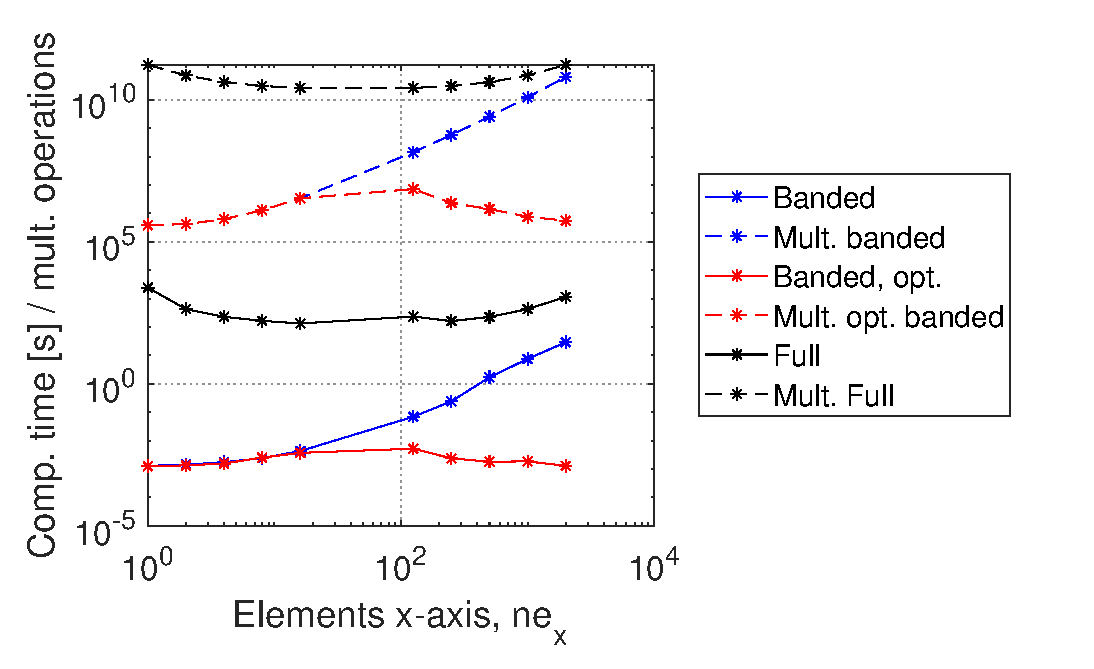
\includegraphics[trim=.0cm .0cm .750cm .0cm, clip=true,width=1\linewidth]{Figures/Plots/ex1plot.eps}
\caption{Logarithmic plot of measured computation time and computational expense various meshes using the banded, full and optimized banded solution.}
\label{fig:ex1plot}
\end{wrapfigure}
The solution was timed for the mesh-variations and plotted  in \Cref{fig:ex1plot}. The shape of the timed solution graph, is compared with the theoretical predictions, measured in multiplication operations. The measured times and theoretical predictions show a similar shape with slight deviations caused by the a varying available computer power. This study does not account for the storage time involved when solving the system. The matrix size determines the necessary amount of numbers to store, which is given by $neqn \times neqn$ and $bw \times neqn$ for full and banded matrices, respectively.

\vspace{-3mm}
\paragraph{1.3}
The bandwidths have been optimized using different combinations of the optimizers \textit{bandfem} and \textit{renum}. The renumbering with the lowest bandwidths is shown in \Cref{tab:equationsolv}. For all meshes where $\text{ne}_x<\text{ne}_y$ the original mesh is the most optimal. For meshes where $\text{ne}_x>\text{ne}_y$ the mesh has been improved after employing \textit{bandfem} and \textit{renum}, which significantly reduced the computation time. The optimizer does not actually find the optimal mesh as it was expected that the bandwidth of mirrored meshes would be equal, e.g. bandwidth of meshes $1000 \times 2$ and $2 \times 1000$ are equal.

\squeezeup
\paragraph{1.4} \Cref{fig:ex1plot} illustrates the calculation time for the optimized meshes (in red) which roughly follows the shape of the theoretical plot. The optimized solution follows the original for the meshes with $\text{ne}_x=[1,2,4,8,16]$. For meshes with $\text{ne}_x=[125,250,500,1000,2000]$ the optimizer renumbered nodes to significantly reduce computation time. The plot is not symmetrical which otherwise was expected if it was not for the optimization issues addressed in \textbf{1.3}.








